%%%%%%%%%%%%%%%%%%%%%%%%%%%%%%%%%%%%
%% PREAMBLE
%%%%%%%%%%%%%%%%%%%%%%%%%%%%%%%%%%%%

\documentclass[11pt]{article}

% packages needed for state diagrams
\usepackage{pgf}
\usepackage{tikz}
\usetikzlibrary{arrows,automata,positioning}

% nice clickable URLs
\usepackage{url}
\usepackage{amssymb}

% page margins
\usepackage[margin=2.5cm]{geometry}
\setlength{\parindent}{0pt}

\begin{document}

%%%%%%%%%%%%%%%%%%%%%%%%%%%%%%%%%%%%
%% HEADING
%%%%%%%%%%%%%%%%%%%%%%%%%%%%%%%%%%%%

\rule{\textwidth}{1pt}
\begin{center}
  \textbf{Taaltheorie en Taalverwerking -- Homework Submission}
\end{center}
\rule{\textwidth}{0.5pt}\\

%%%%%%%%%%%%%%%%%%%%%%%%%%%%%%%%%%%%
%% ENTER DETAILS
%%%%%%%%%%%%%%%%%%%%%%%%%%%%%%%%%%%%

\textbf{Week:} 1

\textbf{Group:} 28

\textbf{Student names and IDs:} Bob Engel 12627143, Dion Streefkerk 15847195

\textbf{Date:} April 8, 2026

\rule{\textwidth}{1pt}

%%%%%%%%%%%%%%%%%%%%%%%%%%%%%%%%%%%%
%% YOUR ANSWERS
%%%%%%%%%%%%%%%%%%%%%%%%%%%%%%%%%%%%

\begin{enumerate}

%% ========== EXERCISE 1 ==========
\item \textbf{Regular expression membership}

\begin{enumerate}

%% 1a
\item $xy(z)^*(zyx)^+$ over $\Sigma_1 = \{x, y, z\}$.

The string must start with $xy$, then zero or more $z$'s, then one or more repetitions of $zyx$.

\begin{tabular}{lll}
1. $\epsilon$ & No & (missing $xy$ and at least one $zyx$) \\
2. $xyz$ & No & (no complete $zyx$ block) \\
3. $xyzyx$ & Yes & ($xy \cdot \epsilon \cdot zyx$) \\
4. $xyzzzyx$ & Yes & ($xy \cdot zz \cdot zyx$) \\
5. $xyzyxzyx$ & Yes & ($xy \cdot \epsilon \cdot zyx \cdot zyx$) \\
6. $xyzzzz$ & No & (no $zyx$ at the end) \\
\end{tabular}

\textbf{Accepted: 3, 4, 5}

%% 1b
\item $yeah(yeah \mid h)^*$ over $\Sigma_2 = \{a, b, c, \ldots, x, y, z\}$.

The string must start with $yeah$, followed by zero or more repetitions of $yeah$ or $h$.

\begin{tabular}{lll}
1. $\epsilon$ & No & (missing initial $yeah$) \\
2. $yeah$ & Yes & ($yeah \cdot \epsilon$) \\
3. $yeahh$ & Yes & ($yeah \cdot h$) \\
4. $hyeah$ & No & (does not start with $yeah$) \\
5. $yeahhyeahh$ & Yes & ($yeah \cdot h \cdot yeah \cdot h$) \\
6. $yeahyeahyeahyeahyeah$ & Yes & ($yeah \cdot yeah \cdot yeah \cdot yeah \cdot yeah$) \\
\end{tabular}

\textbf{Accepted: 2, 3, 5, 6}

%% 1c
\item $((yeahyeah)^* \mid (h)^*)$ over $\Sigma_2 = \{a, b, c, \ldots, x, y, z\}$.

This is a disjunction: either zero or more repetitions of $yeahyeah$, or zero or more $h$'s.

\begin{tabular}{lll}
1. $\epsilon$ & Yes & (either branch with 0 repetitions) \\
2. $yeah$ & No & (not a multiple of $yeahyeah$, not only $h$'s) \\
3. $yeahhhh$ & No & (mix of letters and $h$'s, fits neither branch) \\
4. $yeahhhyeahh$ & No & (fits neither branch) \\
5. $yeahyeahyeahyeah$ & Yes & ($yeahyeah \cdot yeahyeah$) \\
6. $yeahyeahyeahyeahyeah$ & No & (5 $\times$ $yeah$ is not divisible into pairs) \\
\end{tabular}

\textbf{Accepted: 1, 5}

\end{enumerate}

%% ========== EXERCISE 2 ==========
\item \textbf{Writing regular expressions}

\begin{enumerate}

%% 2a
\item The set of all alphabetic strings.

$\Sigma = \{a, b, c, \ldots, z, A, B, \ldots, Z\}$

Mathematical: $\Sigma^*$

Perl/Python:
\begin{verbatim}
/^[a-zA-Z]*$/
\end{verbatim}

%% 2b
\item All non-empty strings over $\Sigma = \{a, b\}$ such that each $a$ is immediately preceded by and immediately followed by a $b$.

Every $a$ must be sandwiched between $b$'s, so the string always starts and ends with $b$, and $a$'s never appear consecutively.

Mathematical: $b^+(ab^+)^*$

Perl/Python:
\begin{verbatim}
/^b+(ab+)*$/
\end{verbatim}

%% 2c
\item All strings that start at the beginning of the line with an integer and end at the end of the line with a word.

$\Sigma = \{0\text{--}9, a\text{--}z, A\text{--}Z, \text{space}, \text{punctuation}, \ldots\}$

Mathematical: $[0\text{-}9]^+ \Sigma^* [a\text{-}zA\text{-}Z]^+$

Perl/Python:
\begin{verbatim}
/^\d+.*[a-zA-Z]+$/
\end{verbatim}

%% 2d
\item All strings that have both the word \emph{flower} and the word \emph{bee} in them as whole words.

$\Sigma = \{a\text{--}z, A\text{--}Z, \text{space}, \text{punctuation}, \ldots\}$

Both orderings (flower before bee, or bee before flower) must be covered.

Mathematical: $\Sigma^* \text{\textbackslash b} flower \text{\textbackslash b} \Sigma^* \text{\textbackslash b} bee \text{\textbackslash b} \Sigma^* \mid \Sigma^* \text{\textbackslash b} bee \text{\textbackslash b} \Sigma^* \text{\textbackslash b} flower \text{\textbackslash b} \Sigma^*$

Perl/Python:
\begin{verbatim}
/^.*\bflower\b.*\bbee\b.*$|^.*\bbee\b.*\bflower\b.*$/
\end{verbatim}

\end{enumerate}

%% ========== EXERCISE 3 ==========
\item \textbf{Non-deterministic FSA}

\begin{enumerate}

%% 3a
\item The machine is non-deterministic because state $q_1$ has two outgoing transitions with the same symbol $b$: one self-loop back to $q_1$ and one to $q_2$. When reading $b$ in state $q_1$, it is not uniquely determined which state the machine transitions to.

%% 3b
\item Tracing each string (the basic path is $q_0 \xrightarrow{a} q_1 \xrightarrow{b} q_2 \xrightarrow{a} q_3$, with self-loops $q_1 \xrightarrow{b} q_1$ and accepting state $q_3$ having no outgoing transitions):

\begin{tabular}{lll}
(i) $aba$ & Accepted & $q_0 \xrightarrow{a} q_1 \xrightarrow{b} q_2 \xrightarrow{a} q_3$ \\
(ii) $abbba$ & Accepted & $q_0 \xrightarrow{a} q_1 \xrightarrow{b} q_1 \xrightarrow{b} q_1 \xrightarrow{b} q_2 \xrightarrow{a} q_3$ \\
(iii) $abaaba$ & Not accepted & stuck in $q_3$ after 3 symbols \\
(iv) $abaababa$ & Not accepted & stuck in $q_3$ after 3 symbols \\
(v) $abbbaabbba$ & Not accepted & stuck in $q_3$ after 5 symbols \\
\end{tabular}

\textbf{Not accepted: (iii), (iv), (v)}

%% 3c
\item We add a transition $q_3 \xrightarrow{a} q_1$ so that the pattern $ab^+a$ can be repeated.

\begin{center}
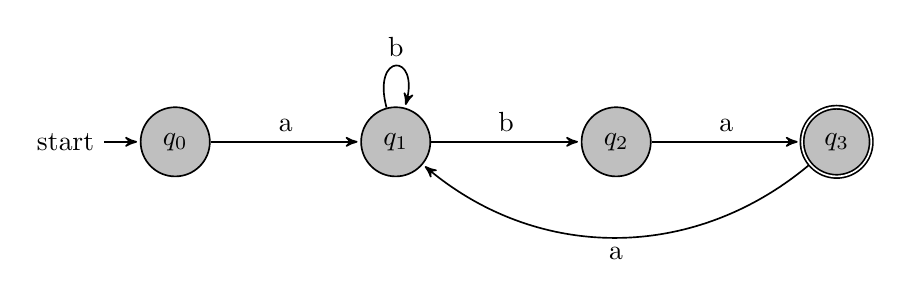
\begin{tikzpicture}[->,>=stealth',shorten >=1pt,auto,node distance=2.8cm,semithick]
  \tikzstyle{every state}=[fill=lightgray,draw=black,text=black]
\node[initial,state] (q0) {$q_0$};
\node[state] (q1) [right of=q0] {$q_1$};
\node[state] (q2) [right of=q1] {$q_2$};
\node[state,accepting] (q3) [right of=q2] {$q_3$};
\path
(q0) edge node {a} (q1)
(q1) edge node {b} (q2)
(q1) edge [loop above] node {b} (q1)
(q2) edge node {a} (q3)
(q3) edge [bend left=40] node [below] {a} (q1);
\end{tikzpicture}
\end{center}

Verification: $abaaba$: $q_0 \xrightarrow{a} q_1 \xrightarrow{b} q_2 \xrightarrow{a} q_3 \xrightarrow{a} q_1 \xrightarrow{b} q_2 \xrightarrow{a} q_3$ \checkmark \\
$abaababa$: $q_0 \xrightarrow{a} q_1 \xrightarrow{b} q_2 \xrightarrow{a} q_3 \xrightarrow{a} q_1 \xrightarrow{b} q_2 \xrightarrow{a} q_3 \xrightarrow{a} q_1 \xrightarrow{b} q_2 \xrightarrow{a} q_3$ \checkmark \\
$abbbaabbba$: $q_0 \xrightarrow{a} q_1 \xrightarrow{b} q_1 \xrightarrow{b} q_1 \xrightarrow{b} q_2 \xrightarrow{a} q_3 \xrightarrow{a} q_1 \xrightarrow{b} q_1 \xrightarrow{b} q_1 \xrightarrow{b} q_2 \xrightarrow{a} q_3$ \checkmark

%% 3d
\item The machine accepts one or more repetitions of the pattern $ab^+a$, where the final $a$ of one block overlaps with the initial $a$ of the next block via the $q_3 \to q_1$ transition.

$$(ab^+a)^+$$

\end{enumerate}

%% ========== EXERCISE 4 ==========
\item \textbf{NFSA to DFSA}

\begin{enumerate}

%% 4a
\item The NFSA accepts strings starting with $0$, followed by alternating $10$ pairs, ending with either $1$ or $10$.

Non-determinism: $q_1$ has two transitions with symbol $1$ (to $q_2$ and to $q_3$), and $q_2$ has two transitions with symbol $0$ (to $q_1$ and to $q_3$).

Regular expression:

$$0(10)^*1(0 \mid \epsilon)$$

Verification: $01$ \checkmark, $010$ \checkmark, $0101$ \checkmark, $01010$ \checkmark.

%% 4b
\item Subset construction:

Start state: $\{q_0\}$. Accepting states contain $q_3$.

\begin{itemize}
\item $\{q_0\}$: input $0 \to \{q_1\}$; input $1 \to \emptyset$
\item $\{q_1\}$: input $0 \to \emptyset$; input $1 \to \{q_2, q_3\}$
\item $\{q_2, q_3\}$: input $0 \to \{q_1, q_3\}$ (from $q_2$); input $1 \to \emptyset$
\item $\{q_1, q_3\}$: input $0 \to \emptyset$; input $1 \to \{q_2, q_3\}$
\end{itemize}

Let $A = \{q_0\}$, $B = \{q_1\}$, $C = \{q_2, q_3\}$, $D = \{q_1, q_3\}$. Accepting: $C, D$.

\begin{center}
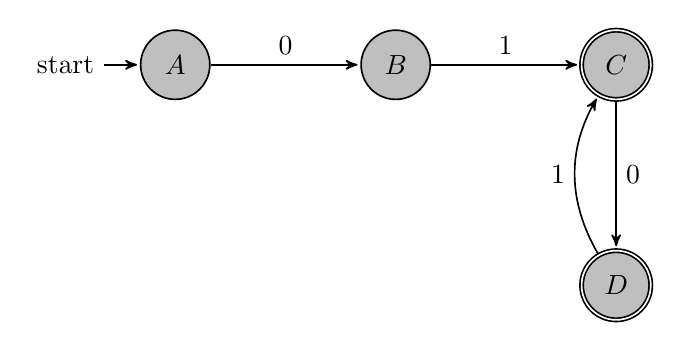
\begin{tikzpicture}[->,>=stealth',shorten >=1pt,auto,node distance=2.8cm,semithick]
  \tikzstyle{every state}=[fill=lightgray,draw=black,text=black]
\node[initial,state] (A) {$A$};
\node[state] (B) [right of=A] {$B$};
\node[state,accepting] (C) [right of=B] {$C$};
\node[state,accepting] (D) [below of=C] {$D$};
\path
(A) edge node {0} (B)
(B) edge node {1} (C)
(C) edge node {0} (D)
(D) edge [bend left] node {1} (C);
\end{tikzpicture}
\end{center}

\end{enumerate}

%% ========== EXERCISE 5 ==========
\item \textbf{FST for Dutch verb \emph{vinden}}

The FST maps all forms \{vind, vindt, vinden, vond, vonden\} to the lemma \emph{vind}.

Key mappings:
\begin{itemize}
\item $vind \to vind$: copy all symbols.
\item $vindt \to vind$: the $t$ maps to $\epsilon$.
\item $vinden \to vind$: the $en$ maps to $\epsilon$.
\item $vond \to vind$: the $o$ maps to $i$.
\item $vonden \to vind$: the $o$ maps to $i$, and $en$ maps to $\epsilon$.
\end{itemize}

\begin{center}
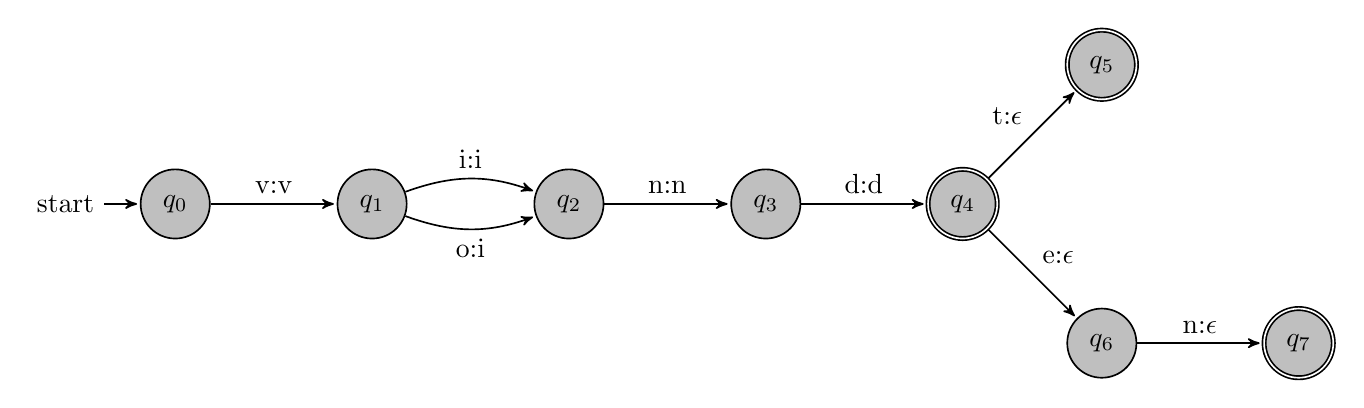
\begin{tikzpicture}[->,>=stealth',shorten >=1pt,auto,node distance=2.5cm,semithick]
  \tikzstyle{every state}=[fill=lightgray,draw=black,text=black]
\node[initial,state] (q0) {$q_0$};
\node[state] (q1) [right of=q0] {$q_1$};
\node[state] (q2) [right of=q1] {$q_2$};
\node[state] (q3) [right of=q2] {$q_3$};
\node[state,accepting] (q4) [right of=q3] {$q_4$};
\node[state,accepting] (q5) [above right of=q4] {$q_5$};
\node[state] (q6) [below right of=q4] {$q_6$};
\node[state,accepting] (q7) [right of=q6] {$q_7$};
\path
(q0) edge node {v:v} (q1)
(q1) edge [bend left=20] node [above] {i:i} (q2)
(q1) edge [bend right=20] node [below] {o:i} (q2)
(q2) edge node {n:n} (q3)
(q3) edge node {d:d} (q4)
(q4) edge node {t:$\epsilon$} (q5)
(q4) edge node {e:$\epsilon$} (q6)
(q6) edge node {n:$\epsilon$} (q7);
\end{tikzpicture}
\end{center}

States: $Q = \{q_0, q_1, q_2, q_3, q_4, q_5, q_6, q_7\}$, start: $q_0$, $F = \{q_4, q_5, q_7\}$.

%% ========== EXERCISE 6 ==========
\item \textbf{Stemming}

\begin{enumerate}

%% 6a
\item Stemming is the process of reducing words to their stem by stripping suffixes (and sometimes prefixes). The goal is to map different inflected or derived forms of the same word to a common base form, so they can be treated as the same token (e.g., for information retrieval). Unlike lemmatization, the resulting stem does not have to be a valid word.

%% 6b
\item Three stemming rules for English:

\textbf{Rule 1:} Remove \texttt{-ing} from the end of a word.\\
Correct: \emph{running} $\to$ \emph{runn}, \emph{walking} $\to$ \emph{walk}.\\
Errors (over-stemming): \emph{king} $\to$ \emph{k}, \emph{ring} $\to$ \emph{r}. Here \emph{-ing} is part of the root, not a suffix.

\textbf{Rule 2:} Remove \texttt{-s} from the end of a word.\\
Correct: \emph{cats} $\to$ \emph{cat}, \emph{runs} $\to$ \emph{run}.\\
Errors (over-stemming): \emph{bus} $\to$ \emph{bu}, \emph{gas} $\to$ \emph{ga}. The \emph{-s} is not a plural or verb suffix here.

\textbf{Rule 3:} Replace \texttt{-ies} with \texttt{-y}.\\
Correct: \emph{ponies} $\to$ \emph{pony}, \emph{berries} $\to$ \emph{berry}.\\
Errors (over-stemming): \emph{series} $\to$ \emph{sery} (but \emph{series} is already singular/plural). \emph{dies} $\to$ \emph{dy} (but the stem should be \emph{die}).

\end{enumerate}

\end{enumerate}


%%%%%%%%%%%%%%%%%%%%%%%%%%%%%%%%%%%%
%% END
%%%%%%%%%%%%%%%%%%%%%%%%%%%%%%%%%%%%

\end{document}
